\section{Rejection-Aware Adaptive Resource Allocation}
\label{sec:stage2_allocator}

\subsection{Role of the Second Stage}

The second stage is applied only after \fedddqn{} selects edge execution. It does not change the edge/cloud decision. Its role is to assign CPU, memory, and bandwidth shares for edge-selected tasks while respecting demand, priority, deadline pressure, and pre-decision QoS/admission risk. This separation keeps the primary contribution focused on task offloading while moving the pipeline closer to an edge resource manager.

Let $\mathcal{I}_e=\{i:a_i=0\}$ denote the set of tasks selected for edge execution. The reported Stage-2 metrics use the filtered allocator-valid set
\[
\mathcal{I}^{\mathrm{valid}}_e=
\{i\in\mathcal{I}_e:\psi_i^{\mathrm{alloc}}=1\},
\]
where $\psi_i^{\mathrm{alloc}}$ marks tasks with complete proxy-target and edge-capacity fields. In the test interval this gives \StageTwoEdgeTasks{} edge-selected allocator-valid tasks out of \StageTwoValidTasks{} \StageTwoFilterRule. This denominator is narrower than the full offloading test split because allocator evaluation requires complete generated proxy-target and edge-capacity fields. For each task, the allocator predicts
\begin{equation}
\hat{\mathbf{y}}_i=\left[\hat{y}^{cpu}_i,\hat{y}^{mem}_i,\hat{y}^{bw}_i\right],
\label{eq:alloc_vector}
\end{equation}
where the three components represent normalized CPU, memory, and bandwidth assignment.
For group-wise normalization, define the active allocator group
\begin{equation}
\mathcal{G}^{\mathrm{valid}}_e(j,t)=
\{\ell\in\mathcal{I}^{\mathrm{valid}}_e:j_\ell=j,\;t_\ell=t\}.
\label{eq:valid_allocator_group}
\end{equation}
This keeps the capacity-normalization denominator tied to the same allocator-valid edge-selected set used for evaluation.

\subsection{Demand-Proportional Base Allocation}

The allocator begins with a demand-proportional base vector $\mathbf{b}_i$. This base allocation is a reasonable first estimate because larger tasks generally need more compute and memory. Demand alone is not enough, however. A high-priority emergency task with a tight deadline can need a different allocation than a low-priority task with similar size. A task with higher QoS/admission risk may also require a conservative correction to avoid under-allocation.

The base vector can be written component-wise as
\begin{equation}
\begin{aligned}
b_i^{cpu} &=
\frac{c_i}{\sum_{\ell\in\mathcal{G}^{\mathrm{valid}}_e(j_i,t_i)}c_\ell},\\
b_i^{mem} &=
\frac{m_i}{\sum_{\ell\in\mathcal{G}^{\mathrm{valid}}_e(j_i,t_i)}m_\ell},\\
b_i^{bw} &=
\frac{d_i}{\sum_{\ell\in\mathcal{G}^{\mathrm{valid}}_e(j_i,t_i)}d_\ell}.
\end{aligned}
\label{eq:base_alloc}
\end{equation}
where $\mathcal{G}^{\mathrm{valid}}_e(j_i,t_i)$ is the allocator-valid active group competing for edge node $j_i$ at time $t_i$. The implementation uses normalized feature inputs and generated proxy targets, while the equation gives the allocation intuition.

\subsection{Generated QoS-Aware Allocation Targets}

The allocator targets are generated proxy targets, not measured optimal allocations from a deployed cluster. Let
\begin{equation}
\mathbf{y}_i^{*}=
\left[y_i^{*,cpu},y_i^{*,mem},y_i^{*,bw}\right]
\label{eq:allocator_target_vector}
\end{equation}
denote the generated CPU, memory, and bandwidth proxy target. These targets are built from observable task and state fields so that training reflects demand, urgency, local contention, channel stress, and reliability risk without using the final allocation prediction as its own label. The deadline term is converted into a tightness score before it enters the allocator:
\begin{equation}
\bar{\delta}_i=
\mathrm{clip}_{[0,1]}\left(
\frac{\delta_{\max}-\delta_i}{\delta_{\max}-\delta_{\min}+\epsilon}
\right),
\label{eq:deadline_tightness}
\end{equation}
so larger $\bar{\delta}_i$ means a tighter deadline rather than a longer one. A compact version of the urgency score is
\begin{equation}
u_i^{\mathrm{urg}}=\mathrm{clip}_{[0,1]}
\left(0.30\bar{p}_i+0.45\bar{\delta}_i+0.35\chi_i^{\mathrm{rt}}+0.45e_i^{\mathrm{emg}}\right),
\label{eq:allocator_urgency}
\end{equation}
where $\bar{p}_i$ is normalized priority, $\bar{\delta}_i$ is the deadline-tightness score from Eq.~\eqref{eq:deadline_tightness}, $\chi_i^{\mathrm{rt}}$ is the real-time flag, and $e_i^{\mathrm{emg}}$ is the emergency-task flag. Local queue and network stress are summarized as
\begin{align}
s^q_i &= \mathrm{clip}_{[0,1]}\left(q^e_{j_i,t_i}/80\right),\\
s^n_i &= \mathrm{clip}_{[0,1]}\left(0.45g_t+0.55v_t+0.80o_t+2\ell_t\right),
\label{eq:allocator_stress}
\end{align}
where $g_t$, $v_t$, $o_t$, and $\ell_t$ denote congestion, jitter-storm, outage, and packet-loss indicators. The generated target increases resource shares for urgent, high-priority, reliability-sensitive, low-battery, dependency-heavy, and network-stressed cases, while keeping all three channels clipped to $[0.01,1.0]$. For example,
\begin{equation}
\begin{aligned}
y^{*,cpu}_i
=\mathrm{clip}_{[0.01,1]}\Bigg(
&\frac{c_i}{\max(u^e_{j_i,t_i},\epsilon)}
\psi^{cpu}_{\kappa_i} \\
&\times(1+0.35u_i^{\mathrm{urg}})
(1+0.25s^q_i)
\Bigg).
\end{aligned}
\label{eq:allocator_cpu_target}
\end{equation}
with analogous memory and bandwidth components in $\mathbf{y}_i^{*}$ using $m_i/m^e_{j_i,t_i}$ and $d_i/B^{\mathrm{eff}}_{t_i}$. The task-type multiplier $\psi^r_{\kappa_i}$ raises CPU and memory for AI/video/image/firmware-like tasks and raises bandwidth for emergency or voice-like tasks. These proxy targets are meant to produce a consistent QoS-aware allocator benchmark; they are not presented as globally optimal resource labels.

\subsection{Residual Correction, Risk Projection, and Capacity Normalization}

The residual allocator predicts a correction instead of an allocation from scratch:
\begin{equation}
\tilde{\mathbf{y}}_i = \mathbf{b}_i + f_{\phi}(z_i),
\label{eq:residual_alloc_main}
\end{equation}
where $z_i$ contains task, state, offloading, and risk features, and $f_{\phi}$ is a neural network. The correction learns when base demand should be raised or lowered because of deadline, priority, QoS/admission risk, or local pressure.

The risk estimate $\hat{\rho}_i$ is computed before observing the realized outcome. It is a QoS/admission-risk score that combines normalized deadline tightness, priority, real-time/emergency flags, low-battery and corruption indicators, local edge pressure, and network or node-state risk into a bounded value in $[0,1]$. It excludes realized labels $M_i$, $R_i$, and $Q_i$, Oracle actions, and the generated proxy target $\mathbf{y}_i^{*}$ from the allocator input. Pre-decision latency estimates may be used as predictors, but realized selected-path outcomes are not fed to the allocator.

The implemented risk projection uses two branches. The residual branch first clips and capacity-normalizes the neural residual output,
\begin{equation}
\mathbf{y}^{\mathrm{res}}_i=
\Pi_{\mathrm{cap}}\!\left(\mathrm{clip}_{[0,1]}(\tilde{\mathbf{y}}_i)\right).
\label{eq:residual_capacity_branch}
\end{equation}
The demand branch starts from bounded demand scores $\mathbf{d}^{\mathrm{raw}}_i$ and raises support for urgent or high-risk tasks using
\begin{equation}
\omega_i=\mathrm{clip}_{[0.5,3.0]}
\left(1+0.55\rho_i^{\mathrm{sla}}+0.35u_i^{\mathrm{urg}}\right),
\label{eq:risk_demand_weight}
\end{equation}
where $\rho_i^{\mathrm{sla}}$ is the pre-decision edge-SLA-risk component and $u_i^{\mathrm{urg}}$ is the urgency score defined in Eq.~\eqref{eq:allocator_urgency}. The rejection-aware demand branch is
\begin{equation}
\mathbf{y}^{\mathrm{dem}}_i=
\Pi_{\mathrm{cap}}\!\left(\omega_i\mathbf{d}^{\mathrm{raw}}_i\right).
\label{eq:risk_demand_branch}
\end{equation}
The final risk-projected allocation then blends the two capacity-safe branches and normalizes again:
\begin{equation}
\mathbf{y}^{risk}_i=
\Pi_{\mathrm{cap}}\!\left(
0.10\mathbf{y}^{\mathrm{res}}_i+
0.90\mathbf{y}^{\mathrm{dem}}_i
\right).
\label{eq:risk_projection_detail}
\end{equation}
Thus deadline and priority enter through the urgency and QoS/admission-risk features rather than disappearing from the implementation path. Capacity normalization then projects the allocation back into feasible edge capacity:
\begin{equation}
\hat{\mathbf{y}}_i = \Pi_{\mathrm{cap}}(\mathbf{y}^{risk}_i),
\label{eq:cap_projection_main}
\end{equation}
so the final assignments do not exceed normalized node-level limits. Without this projection, a raw neural output can have low average error and still violate capacity on many tasks.

For each resource channel $r\in\{\mathrm{cpu},\mathrm{mem},\mathrm{bw}\}$ and each allocator-valid active edge group $\mathcal{G}^{\mathrm{valid}}_e(j,t)$, the normalization can be written as
\begin{equation}
\hat{y}_{i,r} =
y^{risk}_{i,r}
\min\left(1,\frac{C^r_{j,t}}{\sum_{\ell\in\mathcal{G}^{\mathrm{valid}}_e(j,t)}y^{risk}_{\ell,r}+\epsilon}\right),
\label{eq:cap_norm_detail}
\end{equation}
where $C^r_{j,t}$ is normalized available capacity and $\epsilon$ avoids division by zero. The implementation applies the equivalent scaling operation group-wise, so capacity feasibility is enforced after the neural residual and risk correction.

\begin{figure*}[!t]
\centering
\fbox{\begin{minipage}{0.95\textwidth}
\textbf{Algorithm 3: Rejection-Aware Residual Resource Allocation}\\[0.35em]
\textbf{Input:} edge-selected tasks $\mathcal{I}_e$, task/resource features, demand-proportional base allocation $\mathbf{b}_i$, trained residual network $f_{\phi}$.\\
\textbf{Output:} capacity-feasible allocation $\hat{\mathbf{y}}_i$ for CPU, memory, and bandwidth.\\[0.35em]
1) For each edge-selected task, compute the demand-proportional base allocation $\mathbf{b}_i$.\\
2) Concatenate task descriptors, edge state, network state, policy outputs, and the bounded pre-decision QoS/admission-risk estimate $\hat{\rho}_i$ into allocator input $z_i$; do not include realized labels $M_i$, $R_i$, $Q_i$, Oracle actions, or generated final allocation targets.\\
3) Predict the residual correction $f_{\phi}(z_i)$ and form $\tilde{\mathbf{y}}_i=\mathbf{b}_i+f_{\phi}(z_i)$.\\
4) Build the rejection-aware demand branch from urgency, deadline, priority, edge-SLA risk, and related pre-decision risk features; blend it with the capacity-normalized residual branch.\\
5) Project the result into valid normalized capacity so CPU, memory, and bandwidth assignments remain feasible.\\
6) Report MAE, under-allocation, waste, capacity violation, estimated SLA risk, and efficiency.
\end{minipage}}
\caption{Stage-2 allocation procedure for tasks already routed to edge execution by \fedddqn.}
\label{alg:stage2_allocator}
\end{figure*}


\begin{figure*}[!t]
\centering
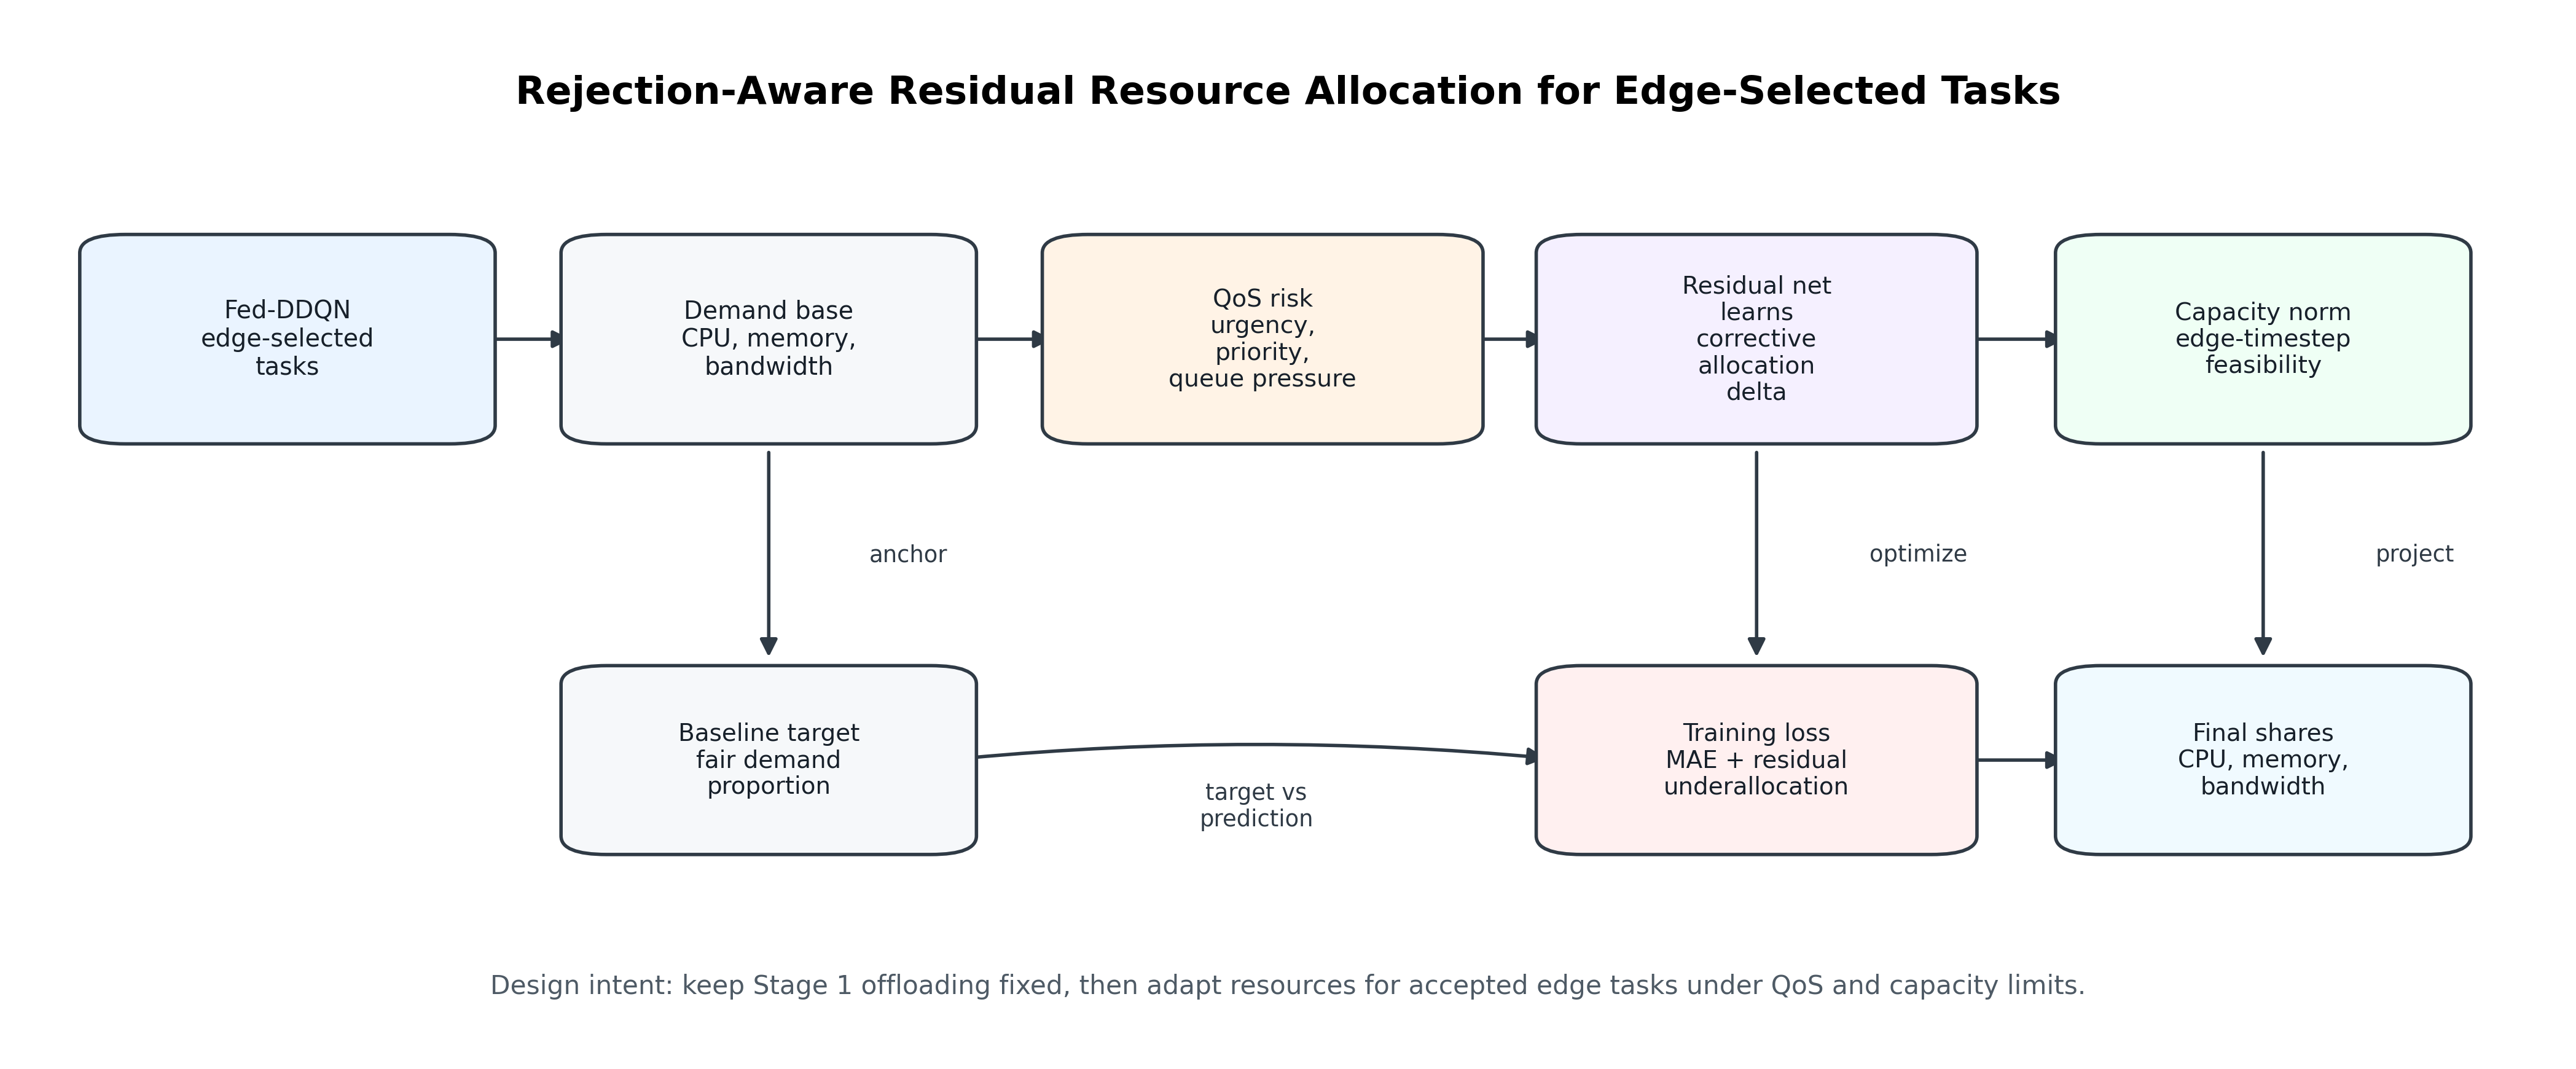
\includegraphics[width=0.88\textwidth]{figures/diagrams/161_fig_a12_stage2_allocator_pipeline.png}
\caption{Rejection-aware residual allocation. A demand-proportional base allocation is corrected by a neural residual, adjusted for risk, and normalized to capacity before evaluation.}
\label{fig:stage2_pipeline}
\end{figure*}

\subsection{Allocator Metrics}

The allocator is evaluated with direct proxy-target error, under-allocation, waste, capacity violation, estimated SLA risk, and an efficiency score on $\mathcal{I}_e^{\mathrm{valid}}$. For generated proxy target $\mathbf{y}_i^{*}$ and predicted final allocation $\hat{\mathbf{y}}_i$, the overall mean absolute error is
\begin{equation}
\mathrm{MAE}=
\frac{1}{3|\mathcal{I}^{\mathrm{valid}}_e|}
\sum_{i\in\mathcal{I}^{\mathrm{valid}}_e}
\lVert \hat{\mathbf{y}}_i-\mathbf{y}_i^{*}\rVert_1.
\label{eq:alloc_mae}
\end{equation}
Under-allocation measures how often the predicted allocation falls below the generated proxy target, while waste measures excess assignment beyond that target. Capacity violation measures whether the combined prediction exceeds normalized node capacity after projection.

The reported allocator result is multi-objective. A method with the lowest proxy-target error may still be undesirable if it produces more under-allocation or capacity violation. In the allocator table, the residual plus risk-projection variant gives the best proxy-target efficiency score while keeping capacity violation at zero.

\subsection{Why the Allocator is Kept Separate}

The allocator could be merged into the offloading policy by expanding the action space to include destination and resource levels. That would be a reasonable future direction, but it would make the current research question less clear. The central question here is whether federated DDQN can learn the edge/cloud decision under channel and QoS stress. If resource allocation were part of the same action, a poor routing decision might be hidden by an allocation correction, or a good routing decision might be penalized because the allocation head was undertrained.

The two-stage structure makes the evaluation easier to read. Stage 1 answers where the task should execute. Stage 2 answers how much edge resource should be assigned after the edge has been chosen. This also matches a common system architecture: a broker selects the execution tier, and a local resource manager performs admission and allocation. The residual allocator is presented as a resource-management companion to the proposed offloading policy, not as a standalone scheduler.
